\chapter{绪论}
\label{chap:myIntro}

\section{研究背景及意义}
\label{sec:background}
增强现实(Augmented Reality,AR)是一种利用计算机生成视觉、听觉等感官信息,与真实世界中的物体进行混合,最终呈现在用户眼前的技术。\cite{ARconception}

目前增强现实广泛应用在诸多领域,例如在游戏领域,增强现实技术可以改变传统游戏的交互方式,为玩家提供新奇的游戏体验。
    
\begin{figure}[!htp]
  \centering
  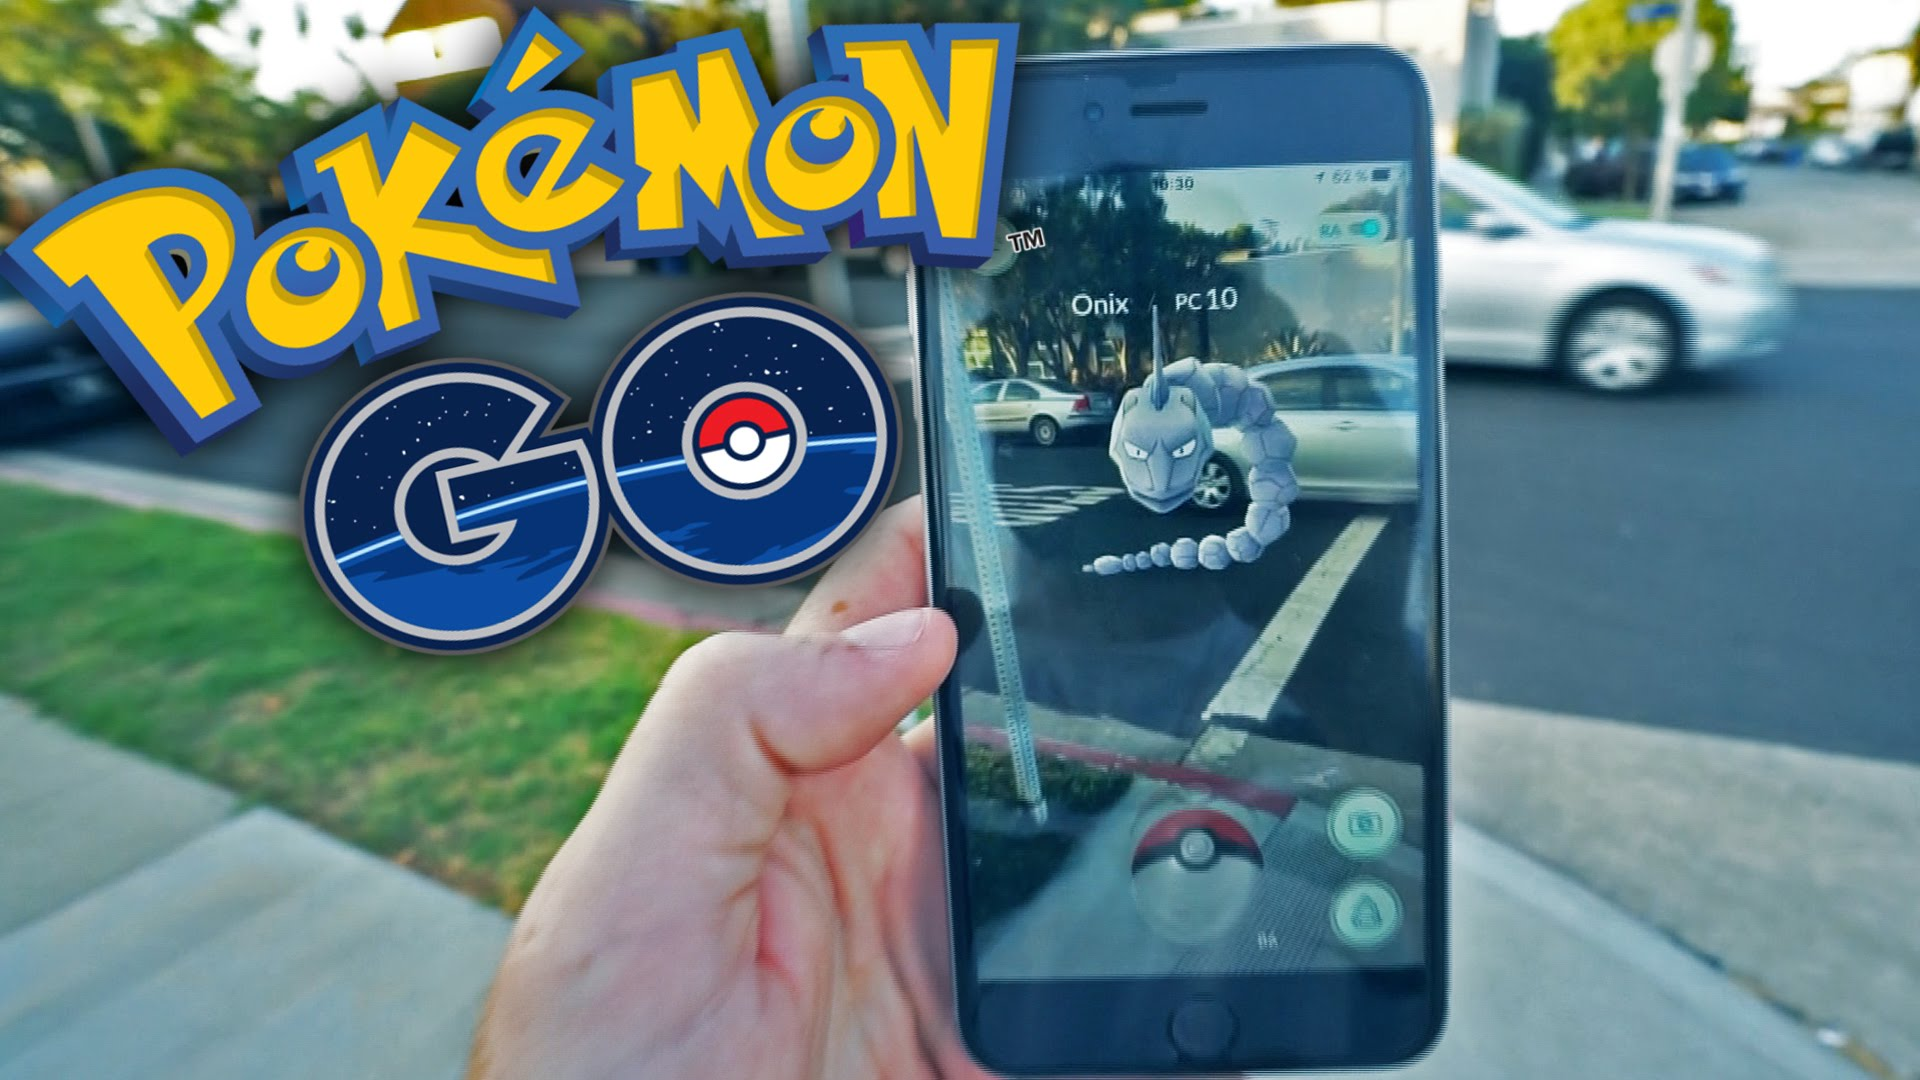
\includegraphics[width=12cm]{pokemongogaming.jpg}
  \bicaption[AR游戏 Pokemon Go海报]
    {AR游戏 Pokemon Go海报}
    {The Poster of AR game Pokemon Go}
 \label{fig:longcaptionbad}
\end{figure}

在工业应用中,可以利用增强现实技术提供辅助信息。例如在汽车领域,增强现实技术能够在驾驶过程中为驾驶员提供导航、路况提醒等功能。\cite{ARdriving}在医学领域,可以通过AR技术将超声波图像显示在患者身体,从而上为手术医生提供信息,辅助医疗。\cite{billinghurst2002augmented}

增强现实技术也逐渐被应用在教育领域,为教师和学生提供更加丰富的教学内容。传统的实验教学存在诸多问题,例如,实验条件(器材、空间、教师、开放时间)有限,学生动手操作和试错的机会少,实验指导不能随着实验进行实时提示与更新等。而增强现实技术因为可以可视化抽象概念,模拟复杂的实验现象,提供实验模拟练习等优势,可以在教学领域得到很好的利用。\cite{wu2013current}但是,教育领域与其他领域不同的是,用户(教育者)也应当是软件开发的一部分,需要具有自主编辑实验的自由。但是教育者由于通常不具备软件开发能力,因此需要应用开发人员提供一套用户友好前端应用,即编著系统。

同时,出于为用户提供更丰富的交互体验,或将虚拟信息与真实物体进行更好融合的目的,需要在增强现实应用中对物体进行识别和追踪。此外,目前的增强现实应用,特别是手机应用,并不能为用户提供真实触感。特别是在教学辅助领域,触感的缺失对于教学质量会有很大的影响。

本项目旨在开发一套增强现实教学辅助应用,在通过后端物体追踪,数据传输,在手机端为用户提供具有真实触感的交互体验,并且在交互过程中利用增强现实技术,显示辅助信息。此外,前端还开发了一套兼容电脑和手机端、用户友好的编著系统,为非计算机专业人士编辑实验教学应用。最终将两个场景融合,使用户在自己编辑完成的实验场景中进行增强现实交互。

这套系统的意义在于,教育者可以在花费较少的学习成本的前提下,自主创建、编辑实验,并且结合现实器材,为学生提供多样的模拟实验。在教学过程中,教育者减少了教学、演示、实验指导的负担,学生实验也可以不受器材、人员等因素的限制,既保证安全,又可以有大量误操作、试错的机会,从而更好地学习如何完成实验。与增强现实技术的结合,使模拟实验更加逼真,学生可以拥有更丰富的学习体验。


\section{国内外研究现状}
\subsection{物体追踪}
目前很多学者在物体追踪方面进行研究。利用已知的物体模型进行追踪的技术可以按照输入图像的种类分为两大类,即利用RGB-D图像和利用RGB图像。每种技术又可以分为物体检测(detection)和物体追踪(tracing)两个步骤。

利用RGB图像进行物体检测的技术,目前使用较多的、可以达到实时速率的是基于模式匹配(template matching)的方法。例如Hinterstoisser等人提出的LINE方法\cite{hinterstoisser2011gradient},在传统的使用图像梯度(gradients)数据检测物体姿态的模式匹配方法的基础上做出改良。他们通过局部优势梯度方向(local dominant gradients orientation)建立模式不变量,并且将梯度方向在图片中的相邻区域也纳入考量范围。将上述两者结合数学表示输入图像,之后进行模式识别,就可以获得更加稳定和高效的追踪效果。此外,近年来也有一些基于机器学习进行物体姿态检测的研究被提出。例如,Brachmann等人提出的,扩展随机森林(random forest)的方法。\cite{brachmann2016uncertainty}但是由于该方法中选择的特征会在很大程度上影响决定姿态的投票的分布,而选择特征往往是一个非常耗时的过程,因此基于随机森林的方法在性能上往往不能满足实时的要求。

而基于RGB图像进行物体追踪的方法,最早能够达到实时要求的是Prisacariu和Reid提出的PWP3D算法\cite{prisacariu2012pwp3d}。该算法构建了一个概率框架,将图象前景部分使用符号距离函数(signed distance function)进行描绘,并且定义了该区域的能量(energy)。而后景部分则基于像素级别的后验隶属概率进行描绘。之后这个方法被Hexer等人发展为利用局部颜色直方图进行前后景分割,提升了效率。\cite{hexner20162d}

仅使用RGB图像进行物体追踪的技术相比于RGB-D图像仍然有所欠缺。例如LINE方法\cite{hinterstoisser2011gradient}在有深度信息时,可以通过获得物体的表面法向量来进一步提升鲁棒性。而Brachmann的方法\cite{brachmann2016uncertainty}通过边缘化物体坐标分布的深度值,从而弥补图像深度值的缺失。相比之下,结合深度值的方法更加成熟与稳定。

在使用RGB-D图像进行物体检测方面,传统的方式可以分为基于模式和基于特征两种。上述的基于模式匹配的LINE方法\cite{hinterstoisser2011gradient}在加入深度信息辅助之后实现的Line-3D,以及其他的类似方法\cite{kehl2016hashmod, rios2013discriminatively}, 都可以实现基于RGB-D图像的物体姿态检测。但是这些方法在检测多个物体时,计算率呈线性增长的,可扩展性差。而基于特征的方法,最早通过RGB图像获得特征\cite{lowe2004distinctive},然后反向投影到三维坐标中的\cite{lowe2001local}。在三维描述符引入后,可以直接通过三维点云计算特征点\cite{mian2010repeatability},从而获得比较好的可扩展性。但这些方法的性能往往不能达到实时的要求。在机器学习技术发展之后,出现了基于随机森林投票确定物体姿态的方法。\cite{brachmann2016uncertainty, tejani2014latent}前者使用能量函数进行姿态估测,而后者则使用投票机制。在这之后,也出现了基于卷积神经网络(convolutional neutral network, CNN)进行姿态识别的研究\cite{kehl2016deep}.该方法使用了局部取样的RGB-D图像补丁(patch)进行神经网络训练,然后在使用的时候通过补丁描述符进行匹配推测物体姿态。

在物体追踪方面,则要充分利用已知的模型数据。通常流程是,构建表示模型的函数,描绘观测图像和目标图像之间的差别,将构造出的代价函数求解局部最小值,从而确定物体姿态。一种处理图像数据的方式是迭代最近点算法(iterative closest point, ICP)。他的目的是通过找到待配准点云数据(追踪时获取的数据)与参考点云数据(物体模型数据)之间的旋转和平移关系,进行最优匹配。Held实现的物体追踪算法就使用了这个方法。\cite{held20123d}但是在多物体追踪时候该算法往往需要预分割点云,但是该算法分割点云和追踪物体只能使用不同的数学模型,导致计算成本增大,一致性差,在追踪多物体的时候效果并不好。
另一种替代ICP的方法是符号距离函数(Signed Distance Function, SDF)。他描绘了点云和物体模型的关系。本文实现的物体追踪系统使用了Ren等人基于SDF实现的物体追踪算法。\cite{ren2017real}他们通过描绘物体的SDF函数,构造代价函数,求解物体姿态,实现物体追踪。具体算法将会在相关技术中详细分析。

\subsection{虚拟场景中的编著系统}
为了满足用户自主编辑虚拟场景的需求,目前有许多应用面市。例如互联网交互游戏Second life,就提供了编程语言Linden Scripting Language(LSL),使用户通过简单的编程,就可以自定义在虚拟场景中与其他物体的交互方式。\cite{LSLTutorial}在LSL的基础上,有很多应用辅助方便用户进行编程、生成代码导入second life进行虚拟交互,如Particle,Dialog Menu, MiceOnABeam Visual Scripting Tool等等。\cite{zhong2014domain}虽然这些工具一定程度上便利了用户编辑和使用虚拟场景,但是用户仍然需要具备一定的编程能力,距离普通教师教学仍有一定差距。

在这之后,有许多模拟程序被开发,例如Ying Zhong等人开发的化学模拟实验引擎。\cite{zhong2014domain}用户可以创建、编辑、操纵化学实验用具,通过TCP/IP与服务器和数据库交流。该工具具有比较好的易用性,但是体现化学专业知识、提示用户实验操作的部分比较少,交互方式也比较局限,并且只支持电脑端。此外,牛津大学也开发了一款用于教学的化学实验模拟引擎,虽然引擎本身对于化学实验及其原理、实验操作都有比较详细的讲述,但是由于实验演示是将预先录制的视频片段整合进行显示的,因此交互方式更加局限。\cite{OxfordChe}在这之后,Ali等人开发了一套化学实验模拟引擎系统,\cite{ali2014effect}将上述两者整合起来,既支持比较丰富的交互方式,又提供化学知识教学,但是该项目已经比较陈旧,在如今看来仍然有可以改进的部分。除此以外,虚拟场景编著系统也在物理等其他自然科学教学领域有所应用。\cite{daineko2017using}

虽然虚拟场景编著系统已经有所应用,但是从上述软件可以看到,它的交互方式仍然局限在电脑屏幕,而且比较缺乏对于实验环境的编辑。

\section{本文主要工作}
本文设计实现了一套具有真实触感的、用于教育领域的增强现实应用。

\begin{figure}[!htp]
  \centering
  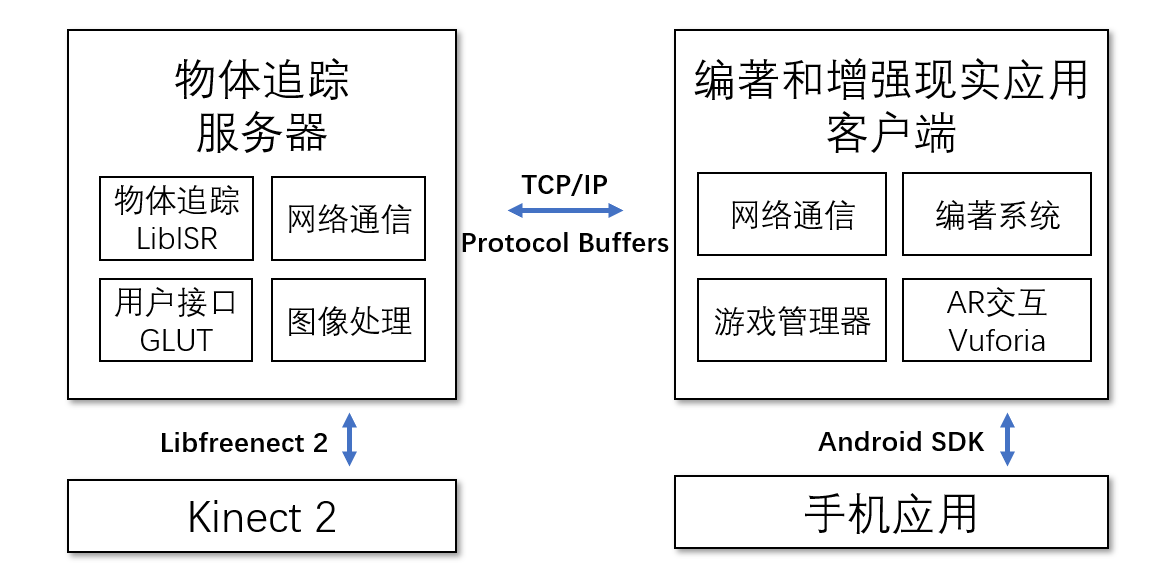
\includegraphics[width=12cm]{figure/work.png}
  \bicaption[本文工作结构图]
    {本文工作结构图}
    {The Structure Diagram of Our Work}
 \label{fig:work}
\end{figure}

应用主要分为客户端和服务器两部分,二者通过网络互传信息。因此,本文工作主要分为服务器、客户端、网络三部分,如图\ref{fig:work}所示。

\begin{itemize}
    \item \textbf{物体追踪服务器}
    
    服务器部分完成的工作主要分为四个部分。图像处理部分通过Libfreenect 2从RGB-D摄像头读取数据,利用标定数据、CUDA加速,将RGB图像和深度图像进行融合。物体追踪部分利用LibISR\cite{Ren_3DV_2014, star3d_iccv_2013},实现物体追踪,获得物体姿态数据。用户接口(UI)同过GLUT实现计算结果显示,获取用户输入等功能。
    
    \item \textbf{编著和增强现实应用客户端}
    
    客户端部分完成的工作也分为四个部分。客户端基于Unity进行开发,游戏管理器负责控制各场景之间的跳转、保存应用使用过程中产生的数据等内容。编著系统实现了实验编著功能,并且提供对应的用户接口。增强现实交互利用编著结果、物体追踪结果、Vuforia平面识别辅助标定进行虚实融合,并且显示模型、文字等虚拟信息。系统还通过Android SDK发布在安卓平台。
    
    \item \textbf{网络通信}
    
    本系统实现了服务器和客户端之间通过网络通信互传数据。服务器和客户端都有对应的网络通信模块,通过Protocol Buffers进行序列化和反序列化数据,TCP/IP协议收发数据,实现用户前端发送指令、服务器返回追踪结果等功能。
    
\end{itemize}


\section{本文结构}
本文一共分为七章。
\begin{itemize}[noitemsep,topsep=0pt,parsep=0pt,partopsep=0pt]
\item 第一章概括介绍了目前增强现实应用的发展背景,物体追踪和编著系统的研究状况,并简单介绍了本文的工作。
\item 第二章着重介绍了项目中使用的技术。首先介绍物体追踪的相关技术,包括Kinect 2的驱动、物体追踪工具及其算法、CUDA架构等内容。之后介绍实现编著系统使用到的技术以及引擎。最后介绍上述两者通信时使用的序列化框架Protocol Buffers和TCP/IP协议等。
\item 第三章分析了项目需求,包括技术需求、用户需求等。之后通过分析、权衡项目需求,完成项目功能设计。
\item 第四章详细介绍了本系统的设计框架。物体追踪服务器按照功能分为四部分分别进行介绍。编著与交互系统客户端按照自顶向下的顺序、逐场景进行阐述。最后介绍两者之间网络通信的框架。
\item 第五章着重从代码和软件层面讲述系统实现。首先介绍了服务器中自主实现的部分,之后按照逐个场景介绍客户端的实现,最后介绍网络通信的实现。
\item 第六章分析了网络传输、物体追踪、增强现实应用的性能数据。然后通过图片辅助展示了系统实现的效果,包括编著系统和增强现实系统。最后简要分析了编著系统的易用性、增强现实应用的使用体验和融合效果等。
\item 最后一章总结全文,总结本系统完成的工作,给出项目存在的缺陷,提出项目未来发展方向。
\end{itemize}
